% WDM package architecture figure
% Compile standalone with tectonic/pdflatex, or copy the tikzpicture into a
% figure environment in the manuscript. Requires: tikz, amsmath, sansmath,
% arrows.meta. A single sans-serif family is used throughout (text and math).
\documentclass[border=4pt]{standalone}
\usepackage{tikz}
\usepackage{amsmath}
\usepackage{sansmath}
\usetikzlibrary{arrows.meta}

% Sans-serif everywhere: text default and math.
\renewcommand{\familydefault}{\sfdefault}
\sansmath

% subtitle text inside boxes and on arrows
\newcommand{\subt}[1]{{\scriptsize\color{black!55}#1}}

\begin{document}
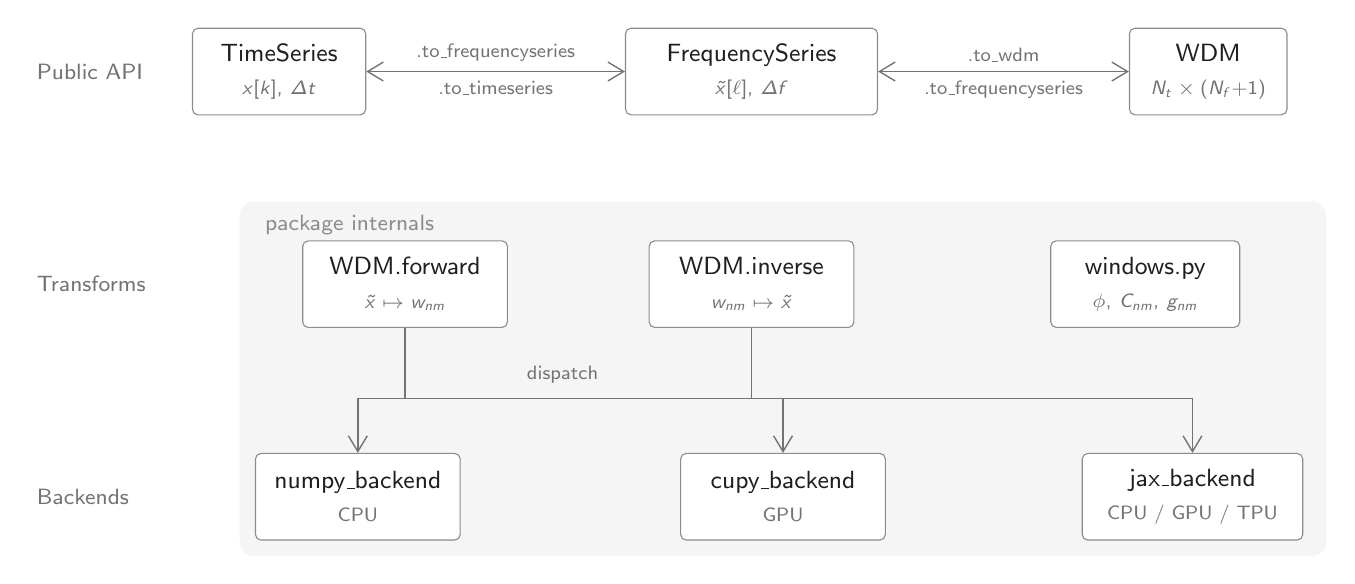
\begin{tikzpicture}[
  font=\sffamily\sansmath\small,
  >={Straight Barb[length=2mm,width=2.4mm]},
  comp/.style={draw=black!45, line width=0.4pt, rounded corners=2pt,
               fill=white, align=center, inner sep=3pt,
               minimum height=11mm, text=black!88},
  zone/.style={font=\sffamily\footnotesize, color=black!55, anchor=west},
  flow/.style={draw=black!55, line width=0.5pt},
]

% --- internal region: filled panel drawn first so it sits behind content ---
\fill[black!4, rounded corners=5pt] (2.9,-0.15) rectangle (16.7,4.35);
\node[font=\sffamily\footnotesize, color=black!45, anchor=west]
      at (3.1,4.05) {package internals};

% --- left-margin section labels ---
\node[zone] at (0.2,6.0) {Public API};
\node[zone] at (0.2,3.3) {Transforms};
\node[zone] at (0.2,0.6) {Backends};

% --- datatypes (public API) ---
\node[comp, minimum width=22mm] (TS) at (3.4,6.0)
      {TimeSeries\\[1pt]\subt{$x[k],\,\Delta t$}};
\node[comp, minimum width=32mm] (FS) at (9.4,6.0)
      {FrequencySeries\\[1pt]\subt{$\tilde{x}[\ell],\,\Delta f$}};
\node[comp, minimum width=20mm] (WD) at (15.2,6.0)
      {WDM\\[1pt]\subt{$N_t\times(N_f{+}1)$}};

% --- transforms ---
\node[comp, minimum width=26mm] (FW) at (5.0,3.3)
      {WDM.forward\\[1pt]\subt{$\tilde{x}\mapsto w_{nm}$}};
\node[comp, minimum width=26mm] (IN) at (9.4,3.3)
      {WDM.inverse\\[1pt]\subt{$w_{nm}\mapsto\tilde{x}$}};
\node[comp, minimum width=24mm] (WN) at (14.4,3.3)
      {windows.py\\[1pt]\subt{$\phi,\,C_{nm},\,g_{nm}$}};

% --- backends (drop cupy here if the package ships NumPy and JAX only) ---
\node[comp, minimum width=26mm] (NP) at (4.4,0.6)
      {numpy\_backend\\[1pt]\subt{CPU}};
\node[comp, minimum width=26mm] (CP) at (9.8,0.6)
      {cupy\_backend\\[1pt]\subt{GPU}};
\node[comp, minimum width=28mm] (JX) at (15.0,0.6)
      {jax\_backend\\[1pt]\subt{CPU / GPU / TPU}};

% --- reversible datatype conversions ---
\draw[flow,<->] (TS.east) --
      node[above]{\subt{.to\_frequencyseries}}
      node[below]{\subt{.to\_timeseries}} (FS.west);
\draw[flow,<->] (FS.east) --
      node[above]{\subt{.to\_wdm}}
      node[below]{\subt{.to\_frequencyseries}} (WD.west);

% --- dispatch bus: transforms feed it, it fans out to the backends ---
\draw[flow] (4.4,1.85) -- (15.0,1.85);
\draw[flow] (FW.south) -- (5.0,1.85);
\draw[flow] (IN.south) -- (9.4,1.85);
\node[font=\sffamily\scriptsize, color=black!55] at (7.0,2.15) {dispatch};
\draw[flow,->] (4.4,1.85) -- (NP.north);
\draw[flow,->] (9.8,1.85) -- (CP.north);
\draw[flow,->] (15.0,1.85) -- (JX.north);

\end{tikzpicture}
\end{document}
